\subsection{Hipotezy Taita}
\label{sub:tait_conjectures}%
\index{hipoteza!Taita|(}%
W tej podsekcji definiujemy stan oraz wygładzenie diagramu, następnie wyprowadzamy wzór o~sumowaniu stanów oraz dowodzimy prawdziwości dwóch technicznych lematów.
Pozwoli to oszacować rozpiętość wielomianu Jonesa, skąd bezpośrednio wynika już I hipoteza Taita \ref{con:tait_1}.
Nie odbiega to znacząco od podejścia Kauffmana w~\cite{kauffman87}.
Na koniec naszkicujemy krótko dowody pozostałych hipotez.

% DICTIONARY;isthmus;przesmyk

\begin{definition}
\index{diagram!zredukowany}%
\index{przesmyk}%
\label{def:isthmus}%
    Wąskie skrzyżowanie między dwiema rozłącznymi częściami diagramu nazywamy przesmykiem.
\begin{comment}
    \[
        \begin{tikzpicture}[baseline=-0.65ex,scale=0.07]
        \begin{knot}[clip width=5]
            \strand[semithick] (-5,-5) rectangle (5,5);
            \strand[semithick] (-5, -3) [in=right, out=left] to (-15, 3);
            \strand[semithick] (-5, 3) [in=right, out=left] to (-15, -3);

            \node at (-20, -3) {$\ldots$};
            \node at (-20,  3) {$\ldots$};
        \end{knot}
        \end{tikzpicture}
    \]
\end{comment}
    Diagram, na którym nie ma żadnych przesmyków, nazywamy zredukowanym.
\end{definition}

Słowo przesmyk pochodzi z teorii grafów, skrzyżowanie jest przesmykiem dokładnie wtedy, gdy odpowiadająca mu krawędź w grafie węzła jest przesmykiem, czyli jej usunięcie zwiększa liczbę składowych spójności.
Tam używa się także określenia most, które u~nas ma już zarezerwowane inne znaczenie.
Poza tym w tej książce nie ma grafów.

\begin{definition}[diagram spójny]
\index{diagram!spójny}%
    Diagram, którego nie można podzielić na dwie niepuste części niespotykające się na żadnym skrzyżowaniu, nazywamy spójnym.
\end{definition}

Jeżeli diagram nie jest spójny, możemy przesunąć rozłączne ogniwa na siebie przy użyciu II ruchu Reidemeistera.
Hipoteza Taita mówi coś o zredukowanych, spójnych i alternujących diagramach.

\begin{definition}[stan]
\index{stan diagramu}%
    Niech $D$ będzie diagramem splotu.
    Każdą funkcję $s$ ze zbioru skrzyżowań diagramu $D$ o wartościach $\pm 1$ nazywamy stanem.
    Sumę wszystkich wartości $s$ oznaczamy $|s|$.
\end{definition}

\begin{definition}
\index{wygładzenie}%
    Niech $D$ będzie diagramem splotu $L$, zaś $s$ jego stanem.
    Diagram powstały przez wygładzenie wszystkich skrzyżowań zgodnie z~ich stanem oznaczamy $sD$.

    Przez $|sD|$ rozumiemy liczbę zamkniętych, nieprzecinających się krzywych, z których składa się nowy diagram.
\end{definition}

\begin{proposition}[o sumowaniu stanów]
\index{wzór o sumowaniu stanów}%
    Niech $D$ będzie diagramem splotu.
    Wtedy
    \begin{equation}
        \langle D\rangle = \sum_s (-A^2-A^{-2})^{|sD|-1} A^{|s|},
    \end{equation}
    gdzie sumujemy po wszystkich stanach $s$ dla diagramu $D$.
\end{proposition}

Dla wygody wprowadźmy skrót $\langle D \mid s \rangle := (-A^{-2}-A^2)^{|sD|-1}A^{|s|}$.

\begin{proof}
    Oznaczmy prawą stronę dowodzonej równości przez $[D]$.
    Pokażemy, że spełnia ona aksjomaty Kauffmana z~definicji \ref{def:kauffman_bracket}, stąd wynika już, że $[D] = \bracket{D}$.
    % ona $[\LittleUnknot]=1$, $[D\sqcup\LittleUnknot]=(-A^{-2}-A^2) [D]$ oraz $[\LittleRightCrossing] = A [\LittleRightSmoothing] + A^{-1}[\LittleLeftSmoothing]$.

    Pierwszy aksjomat (równość \ref{eqn:kauffman_axiom_1}) mówi o niewęźle $\LittleUnknot$.
    Posiada on tylko jeden stan $s$ dany wzorem $|s| = 0$, zatem $|s\,\LittleUnknot| = 1$ oraz $[D] = (-A^2 - A^{-2})^0 \cdot A^0 = 1$.

    By pokazać, że funkcja $[\,\cdot\,]$ spełnia drugi aksjomat (równość \ref{eqn:kauffman_axiom_2}) zauważmy, że diagramy $D \sqcup \LittleUnknot$ oraz $D$ mają te same skrzyżowania,
    więc możemy utożsamiać stany $s$ dla $D$ ze stanami $u$ dla $D \sqcup \LittleUnknot$.
    Wtedy $|u| = |s|$ oraz $|u(D \sqcup \LittleUnknot)| = |sD| + 1$.
    Zatem
    \begin{align}
        \left[D \sqcup \LittleUnknot\right]
        & = \sum_u (-A^2-A^{-2})^{|u(D\sqcup\LittleUnknot)|-1} A^{|u|} \\
        & = \sum_s (-A^2-A^{-2})^{|sD|} A^{|s|} \\
        & = (-A^2-A^{-2}) [D].
    \end{align}
    Pozostał ostatni aksjomat, równość \ref{eqn:kauffman_axiom_3}.
    Bezpośrednio z definicji mamy
    \begin{equation}
       A[\LittleRightSmoothing]
       = \sum_u(-A^2-A^{-2})^{|u\LittleRightSmoothing|-1}A^{|u|+1},
    \end{equation}
    gdzie $u$ przebiega wszystkie stany $\LittleRightSmoothing$.
    Ale $\LittleRightSmoothing$ to $\LittleRightCrossing$ z ustalonym skrzyżowaniem $c$ wygładzonym dodatnio, co daje bijekcję między wszystkimi stanami $u$ diagramu $\LittleRightSmoothing$ oraz tymi stanami $s$ diagramu $\LittleRightCrossing$, dla których $s(c) = + 1$.
    Wtedy $|s\LittleRightCrossing| = |u\LittleRightSmoothing|$, $|s| = |u|+1$ oraz
    \begin{align}
        A\left[\LittleRightSmoothing\right]
        & = \sum_u (-A^2-A^{-2})^{|u\,\LittleRightSmoothing|-1}A^{|u|+1} \\
        \label{eqn:state_sum_right}
        & = \sum_{s(c)=1}(-A^2-A^{-2})^{|s\,\LittleRightCrossing|-1}A^{|s|},
    \end{align}
    podobne rozumowanie pokazuje, że
    \begin{align}
        \label{eqn:state_sum_left}
        A^{-1}\left[\LittleLeftSmoothing\right]
        & = \sum_{s(c)=-1}(-A^2-A^{-2})^{|s\,\LittleRightCrossing|-1}A^{|s|}.
    \end{align}
    Dodanie do siebie równań \ref{eqn:state_sum_right} oraz \ref{eqn:state_sum_left} kończy dowód.
    %: $A[\PrawyGladki]+A^{-1}[\LewyGladki] = \sum_s(-A^2-A^{-2})^{|s\,\LittleRightCrossing|-1}A^{|s|} = [\RightCrossing]$.
\end{proof}
Zbadamy następnie dwa najprostsze stany dowolnego diagramu.

\begin{definition}
    Stan przypisujący wartość $+1$ ($-1$) każdemu skrzyżowaniu oznaczamy $s_+$ ($s_-$).
\end{definition}

Niech $D$ będzie alternującym, zredukowanym diagramem spójnym.
Wtedy wszystkie jego skrzyżowania mają ten sam znak.
Wybierzmy dla niego to uszachowienie, w~którym wszystkie skrzyżowania są dodatnie:
\begin{comment}
\[
    \begin{tikzpicture}[baseline=-0.65ex,scale=0.15]
    \begin{knot}[clip width=5]
        \strand[semithick] (-25, 0) to (25, 0);
        \strand[semithick] (10*0-15, -5) to (10*0-15, 5);
        \strand[semithick] (10*1-15, -5) to (10*1-15, 5);
        \strand[semithick] (10*2-15, -5) to (10*2-15, 5);
        \strand[semithick] (10*3-15, -5) to (10*3-15, 5);
        \draw[fill=blue!10!white,draw=none] (-25, 0) rectangle (-15, -5);
        \draw[fill=blue!10!white,draw=none] (-15, 0) rectangle (-5, 5);
        \draw[fill=blue!10!white,draw=none] (-5, 0) rectangle (5, -5);
        \draw[fill=blue!10!white,draw=none] (5, 0) rectangle (15, 5);
        \draw[fill=blue!10!white,draw=none] (15, 0) rectangle (25, -5);
        \node[above left] at (-15, 0) {$+1$};
        \node[above left] at (5, 0) {$+1$};
        \node[below left] at (-5, 0) {$+1$};
        \node[below left] at (15, 0) {$+1$};
    \end{knot}
    \end{tikzpicture}
\]
\end{comment}
Nazywamy je uszachowieniem \emph{standardowym}.
\index{uszachowienie!standardowe}%
Porównajmy wygładzenie $s_+D$ z~$s_-D$:
\begin{comment}
\[
    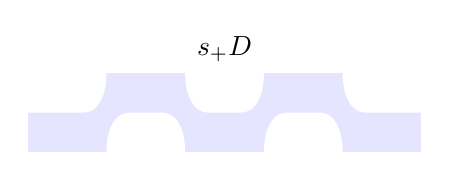
\begin{tikzpicture}[baseline=-0.65ex,scale=0.10]
        \node at (0, 8) {$s_+D$};
        \draw[fill=blue!10!white,draw=none] (-25, -5) rectangle (25, 5);
        \draw[fill=white, draw=none] (-15, -5) [in=left, out=up] to (-12, 0) -- (-8, 0) [in=up, out=right] to (-5, -5);
        \draw[fill=white, draw=none] (5, -5) [in=left, out=up] to (8, 0) -- (12, 0) [in=up, out=right] to (15, -5);
        \draw[fill=white, draw=none] (-5, 5) [in=left, out=down] to (-2, 0) -- (2, 0) [in=down, out=right] to (5, 5);
        \draw[fill=white, draw=none] (-25, 0) -- (-18, 0) [in=down, out=right] to (-15, 5) -- (-25, 5);
        \draw[fill=white, draw=none] ( 25, 0) -- ( 18, 0) [in=down, out=left] to ( 15, 5) -- ( 25, 5);
    \end{tikzpicture}
    \quad
    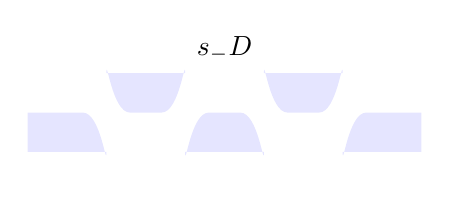
\begin{tikzpicture}[baseline=-0.65ex,scale=0.10]
        \node at (0, 8) {$s_-D$};
        \draw[fill=blue!10!white, draw=none] (-15, 5) [in=left, out=up] to (-12, 0) -- (-8, 0) [in=up, out=right] to (-5, 5);
        \draw[fill=blue!10!white, draw=none] (5, 5) [in=left, out=up] to (8, 0) -- (12, 0) [in=up, out=right] to (15, 5);
        \draw[fill=blue!10!white, draw=none] (-5, -5) [in=left, out=down] to (-2, 0) -- (2, 0) [in=down, out=right] to (5, -5);
        \draw[fill=blue!10!white, draw=none] (-25, 0) -- (-18, 0) [in=down, out=right] to (-15, -5) -- (-25, -5);
        \draw[fill=blue!10!white, draw=none] ( 25, 0) -- ( 18, 0) [in=down, out=left] to ( 15, -5) -- ( 25, -5);
    \end{tikzpicture}
\]
\end{comment}

Zamknięte krzywe tworzące $s_+D$ są brzegami jasnych obszarów uszachowienia, podczas gdy te tworzące $s_-D$ stanowią brzeg ciemnych obszarów.
Zauważmy jeszcze, że na każdym skrzyżowaniu występują cztery różne ciemne i~jasne obszary: gdyby pewien obszar dotykał tam sam siebie, mielibyśmy do czynienia w~tym miejscu z~przesmykiem, a~założyliśmy przecież, że diagram jest zredukowany.

\begin{lemma}
    \label{lem:pretait_lemma_1}
    Niech $D$ będzie spójnym diagramem splotu o~$n$ skrzyżowaniach.
    Wtedy
    \begin{equation}
        |s_+D| + |s_-D| \le n+2,
    \end{equation}
    z~równością, gdy diagram $D$ jest alternujący i~zredukowany.
\end{lemma}

\begin{proof}
    Skorzystamy z~indukcji względem $n$.
    Łatwo widać prawdziwość lematu dla $n = 0$.
    Załóżmy, że jest on prawdziwy dla wszystkich diagramów o~$n - 1$ skrzyżowaniach, następnie ustalmy diagram $D$ o~$n$ skrzyżowaniach.

    Wybierzmy skrzyżowanie na diagramie $D$.
    Można je wygładzić na dwa sposoby, jeden z~nich daje spójny diagram $D'$.
    Bez straty ogólności przyjmijmy, że dzieje się tak podczas dodatniego wygładzenia.
    Wtedy zachodzi $|s_+D'| = |s_+D|$, ale $|s_-D'| = |s_-D|\pm 1$, gdyż diagram $s_-D'$ powstaje z~$s_-D$ po zastąpieniu pewnej części
    $\LittleRightSmoothing$ przez $\LittleLeftSmoothing$.
    To rozrywa jedną krzywą na dwa kawałki lub scala dwie krzywe w~jedną.
    Z założenia indukcyjnego mamy
    \begin{align}
        |s_+D| + |s_-D|
        & = |s_+D'| + |s_-D'| \pm 1 \\
        & \le (n - 1) + 2 \pm 1 \\
        & \le n + 2.
    \end{align}

    Załóżmy, że diagram $D$ jest spójny, alternujący i zredukowany.
    Pierwsza nierówność jest tak naprawdę równością jako powtórzenie założenia indukcynego.
    Z drugiej strony zachodzi $|s_-D'|=|s_-D|-1$, ponieważ przejście od $s_-D$ do $s_-D'$ skleja dwa ciemne obszary, jak na poniższym rysunku:
\begin{comment}
    \[
        \begin{tikzpicture}[baseline=-0.65ex,scale=0.20]
        \begin{knot}[clip width=5]
            \strand[semithick] (-5, 0) to (5, 0);
            \strand[semithick] (0, -5) to (0, 5);
            \draw[fill=blue!10!white,draw=none] (-5, -5) rectangle (0, 0);
            \draw[fill=blue!10!white,draw=none] ( 5,  5) rectangle (0, 0);
            \node at (0, -8) {$D$};
        \end{knot}
        \end{tikzpicture}
        \quad
        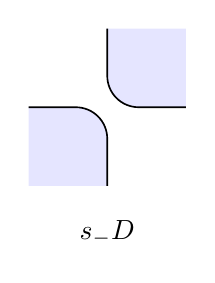
\begin{tikzpicture}[baseline=-0.65ex,scale=0.20]
            \draw[fill=blue!10!white, draw=none] (-5, 0) -- (-2, 0) [in=up, out=right] to (0, -2) -- (0, -5) -- (-5, -5);
            \draw[fill=blue!10!white, draw=none] (5, 0) -- (2, 0) [in=down, out=left] to (0, 2) -- (0, 5) -- (5, 5);
            \draw[semithick] (-5, 0) -- (-2, 0) [in=up, out=right] to (0, -2) -- (0, -5);
            \draw[semithick] (5, 0) -- (2, 0) [in=down, out=left] to (0, 2) -- (0, 5);
            \node at (0, -8) {$s_-D$};
        \end{tikzpicture}
        \quad
        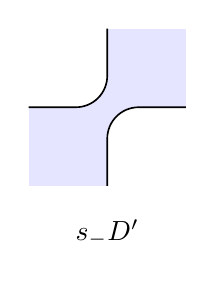
\begin{tikzpicture}[baseline=-0.65ex,scale=0.20]
            \draw[fill=blue!10!white, draw=none] (-5, -5) rectangle (5, 5);
            \draw[fill=white, draw=none] (5, 0) -- (2, 0) [in=up, out=left] to (0, -2) -- (0, -5) -- (5, -5);
            \draw[fill=white, draw=none] (-5, 0) -- (-2, 0) [in=down, out=right] to (0, 2) -- (0, 5) -- (-5, 5);
            \draw[semithick] (5, 0) -- (2, 0) [in=up, out=left] to (0, -2) -- (0, -5);
            \draw[semithick] (-5, 0) -- (-2, 0) [in=down, out=right] to (0, 2) -- (0, 5);
            \node at (0, -8) {$s_-D'$};
        \end{tikzpicture}
    \]
\end{comment}
    Oznacza to, że druga nierówność także jest równością, quod erat demonstrandum.
    \end{proof}

W~dowodzie hipotezy Taita użyjemy rozpiętości wielomianu Jonesa:

\begin{definition}[rozpiętość]
\index{rozpiętość wielomianu}%
    Niech $f$ będzie wielomianem Laurenta jednej zmiennej $X$.
    Różnicę między najwyższą i najniższą potęgą $X$,
    \begin{equation}
        \operatorname{span} f = \operatorname{maxdeg} f - \operatorname{mindeg} f,
    \end{equation}
    nazywamy rozpiętością wielomianu $f$.
\end{definition}

Na przykład $\operatorname{span} (-t+3-1/t) = 1 - (-1) = 2$.

 \begin{lemma}
    \label{lem:pretait_lemma_2}
    Niech $D$ będzie diagramem splotu o~$n$ skrzyżowaniach.
    Wtedy
    \begin{align}
        \operatorname{maxdeg} \langle D \rangle & \le n - 2 + 2|s_+D| \\
        \operatorname{mindeg} \langle D \rangle & \ge 2 - n - 2|s_-D|
    \end{align}
    z równością, jeżeli $D$ jest alternujący, zredukowany i~spójny.
\end{lemma}

\begin{proof}
    Ponieważ dowody tych nierówności przebiegają analogicznie, ograniczymy się do pierwszej z nich.
    Dla oszczędności miejsca będziemy pisać $M$ zamiast $\operatorname{maxdeg}$.

    Niech $s$ będzie dowolnym stanem.
    Istnieje wtedy ciąg stanów $s_+ = s_0, s_1, \ldots, s_r = s$, w~którym stan $s_{i+1}$ powstaje z~$s_i$ przez zmianę wartości w jednym ze skrzyżowań z $+1$ na $-1$.
    Skoro diagram $s_{i+1}D$ uzyskujemy z~$s_{i}D$ przez połączenie dwóch zamkniętych krzywych lub podział jednej krzywej na dwie części, mamy: $|s_{i+1}| = |s_i| - 2$ oraz $|s_{i+1}D| = |s_iD| \pm 1$.
    Wnioskujemy stąd, że
    \begin{align}
        M \langle D \mid s_{i+1} \rangle
        & = 2|s_{i+1}D| + |s_{i+1}|-2 \\
        & = (2|s_iD| + |s_i| -2 ) + (\pm 2-2) \\
        & \le M \langle D|s_i\rangle.
    \end{align}
    Powtarzając odpowiednio wiele razy, dostajemy łańcuch nierówności
    \begin{equation}
        M \langle D \mid s \rangle
        =
        M \langle D \mid s_r \rangle
        \le \ldots \le
        M \langle D \mid s_0 \rangle
        =
        M \langle D \mid s_+ \rangle.
    \end{equation}
    Zauważmy, że dla każdego stanu $s$ zachodzi $M \langle D|s \rangle = 2|sD| + |s| - 2$.
    Zatem
    \begin{equation}
        M \langle D \mid s \rangle \le 2 |s_+D| + |s| - 2 = 2|s_+D| + n - 2,
    \end{equation}
    co kończy dowód pierwszej części lematu.

    Załóżmy teraz, że diagram $D$ jest zredukowany, alternujący i~spójny.
    Chcemy pokazać, że stan $s_+$ dominuje nad pozostałymi: żaden inny nie wnosi do sumy wyrazu z~takim samym najwyższym wykładnikiem.
    Czy warunek $s \neq s_+$ implikuje $M\langle D|s\rangle < M\langle D| s_+\rangle$?
    Dzięki łańcuchowi nierówności wystarczy sprawdzić to tylko dla tych stanów $s$, które powstają z~$s_+$ przez zmianę pojedynczej wartości $+1$ na $-1$.
    Ale to już jest oczywiste, gdyż $sD$ otrzymujemy przez sklejenie dwóch jasnych obszarów $s_+ D$.
\end{proof}

Możemy wreszcie zająć się rozpiętością wielomianu Jonesa.

\begin{proposition}
    Niech $L$ będzie zorientowanym splotem o~spójnym diagramie $D$ z~$n$ skrzyżowaniami.
    Wtedy $\operatorname{span} \jones(L) \le n$, z~równością dla zredukowanego i~alternującego $D$.
\end{proposition}

\begin{proof}
    Pokażemy prawdziwość innego, równoważnego stwierdzenia: $\operatorname{span} \langle D\rangle\le 4n$.
    Dwa poprzednie lematy \ref{lem:pretait_lemma_1} oraz \ref{lem:pretait_lemma_2} mówią razem, że
    \begin{align}
        \operatorname{span}\langle D\rangle
        & = M\langle D\rangle - m\langle D\rangle \\
        & \le (2|s_+D|+n-2)+(2|s_-D|+n-2) \\
        & = 2(|s_+D|+|s_- D|)+2n-4 \\
        & \le 2(n+2)+2n-4 \\
        & = 4n. \qedhere
    \end{align}
\end{proof}

\begin{conjecture}[Taita, pierwsza]
    \index{hipoteza!Taita}
    Zredukowany, spójny, alternujący diagram $D$ zorientowanego splotu $L$ realizuje jego indeks skrzyżowaniowy.
\end{conjecture}

\begin{proof}
    Załóżmy nie wprost, że istnieje diagram o~mniejszej liczbie skrzyżowań,
    mielibyśmy $\operatorname{span} (\jones(L)) < n$, co prowadzi do sprzeczności z~równością $\operatorname{span} (\jones(L)) = n$.
\end{proof}

Szukanie wielomianu Jonesa splotu bywa uciążliwe,
jednak czasami możemy oszacować jego rozpiętość korzystając z~następujących nierówności:

\begin{corollary}
    Niech $L$ będzie zorientowanym splotem ze spójnym diagramem $D$, na którym widać $n$ skrzyżowań.
    Wtedy
    \begin{align}
        3w(D) - 2|s_+D| + 2 - n & \le 4 m(\jones(L) \\
        3w(D) + 2|s_-D| + n - 2 & \ge 4 M(\jones(L)),
    \end{align}
    z~równością dla zredukowanego i~alternującego $D$.
\end{corollary}

\begin{proof}
    Wystarczy powołać się na definicję \ref{def:jones_polynomial} oraz lemat \ref{lem:pretait_lemma_2}.
\end{proof}

Jesteśmy gotowi przejść do kolejnej hipotezy Taita, wciąż podążając za pracą Kauffmana \cite{kauffman87}.
(do napisania)

Dowód trzeciej hipotezy nie zostanie podany.
Korzysta z geometrycznych i algebraicznych technik: pracy Menasco o czterokrotnie przekłutej 2-sferze w dopełnieniu splotu, z własności wielomianów $\jones$ oraz $F$ znalezionych przez Thistlethwaite'a oraz nieściśliwych powierzchnii z~niepołudnikowym brzegiem...

Czwarta hipoteza wynika dla alternujących węzłów z drugiej, ponieważ odbicie lustrzane diagramu zamienia ze sobą dodatnie i ujemne skrzyżowania, a zatem neguje spin.
Założenia, że węzeł jest alternujący nie można pominąć, patrz tekst za przykładem \ref{property_of_eight_knot}.

\begin{proposition}
    Dla każdego nieparzystego $n \ge 15$ istnieje pierwszy, zwierciadlany węzeł $K$, którego indeksem skrzyżowaniowym jest $n$.
\end{proposition}

Dziesięć lat temu Stojmenow zamieścił na portalu arXiv pracę \cite{stoimenow07}; czekam na publikację w recenzowanym czasopiśmie.

\index{hipoteza!Taita|)}%

% Koniec podsekcji Rozpiętość i~wielomian Jonesa
